% Indicate the main file. Must go at the beginning of the file.
% !TEX root = ../main.tex

%----------------------------------------------------------------------------------------
% CHAPTER TEMPLATE
%----------------------------------------------------------------------------------------


\chapter{Conclusion} % Main chapter title

\label{Chapter5} % Change X to a consecutive number; for referencing this chapter elsewhere, use \ref{ChapterX}

%----------------------------------------------------------------------------------------
% SECTION 1
%----------------------------------------------------------------------------------------

\section{Limits on simulation data driven approaches}

\subsection{Overfitting}
% missing the perfect simulation parameters --> deep learning approach!
Using simulated data as training data is an approach which intrinsically needs to be questioned. Under the assumption that the simulation approach used is accurate enough to explain the effects under investigation, we could argue that this effectively solves the task. However, this almost never holds for complex tasks such as ours and thus we expect overfitting on the experimental data.
The process of learning the domain shift between simulated and experimental spectra is commonly referred to as learning the domain shift. To visualize this, Figure \ref{fig:overfit} shows how the model trained on solely uncontaminated (\emph{cont} dataset) data compares to the dataset with a variety of contamination layer thicknesses (\emph{mixcont} dataset).

%   \begin{figure}
%       \centering
%       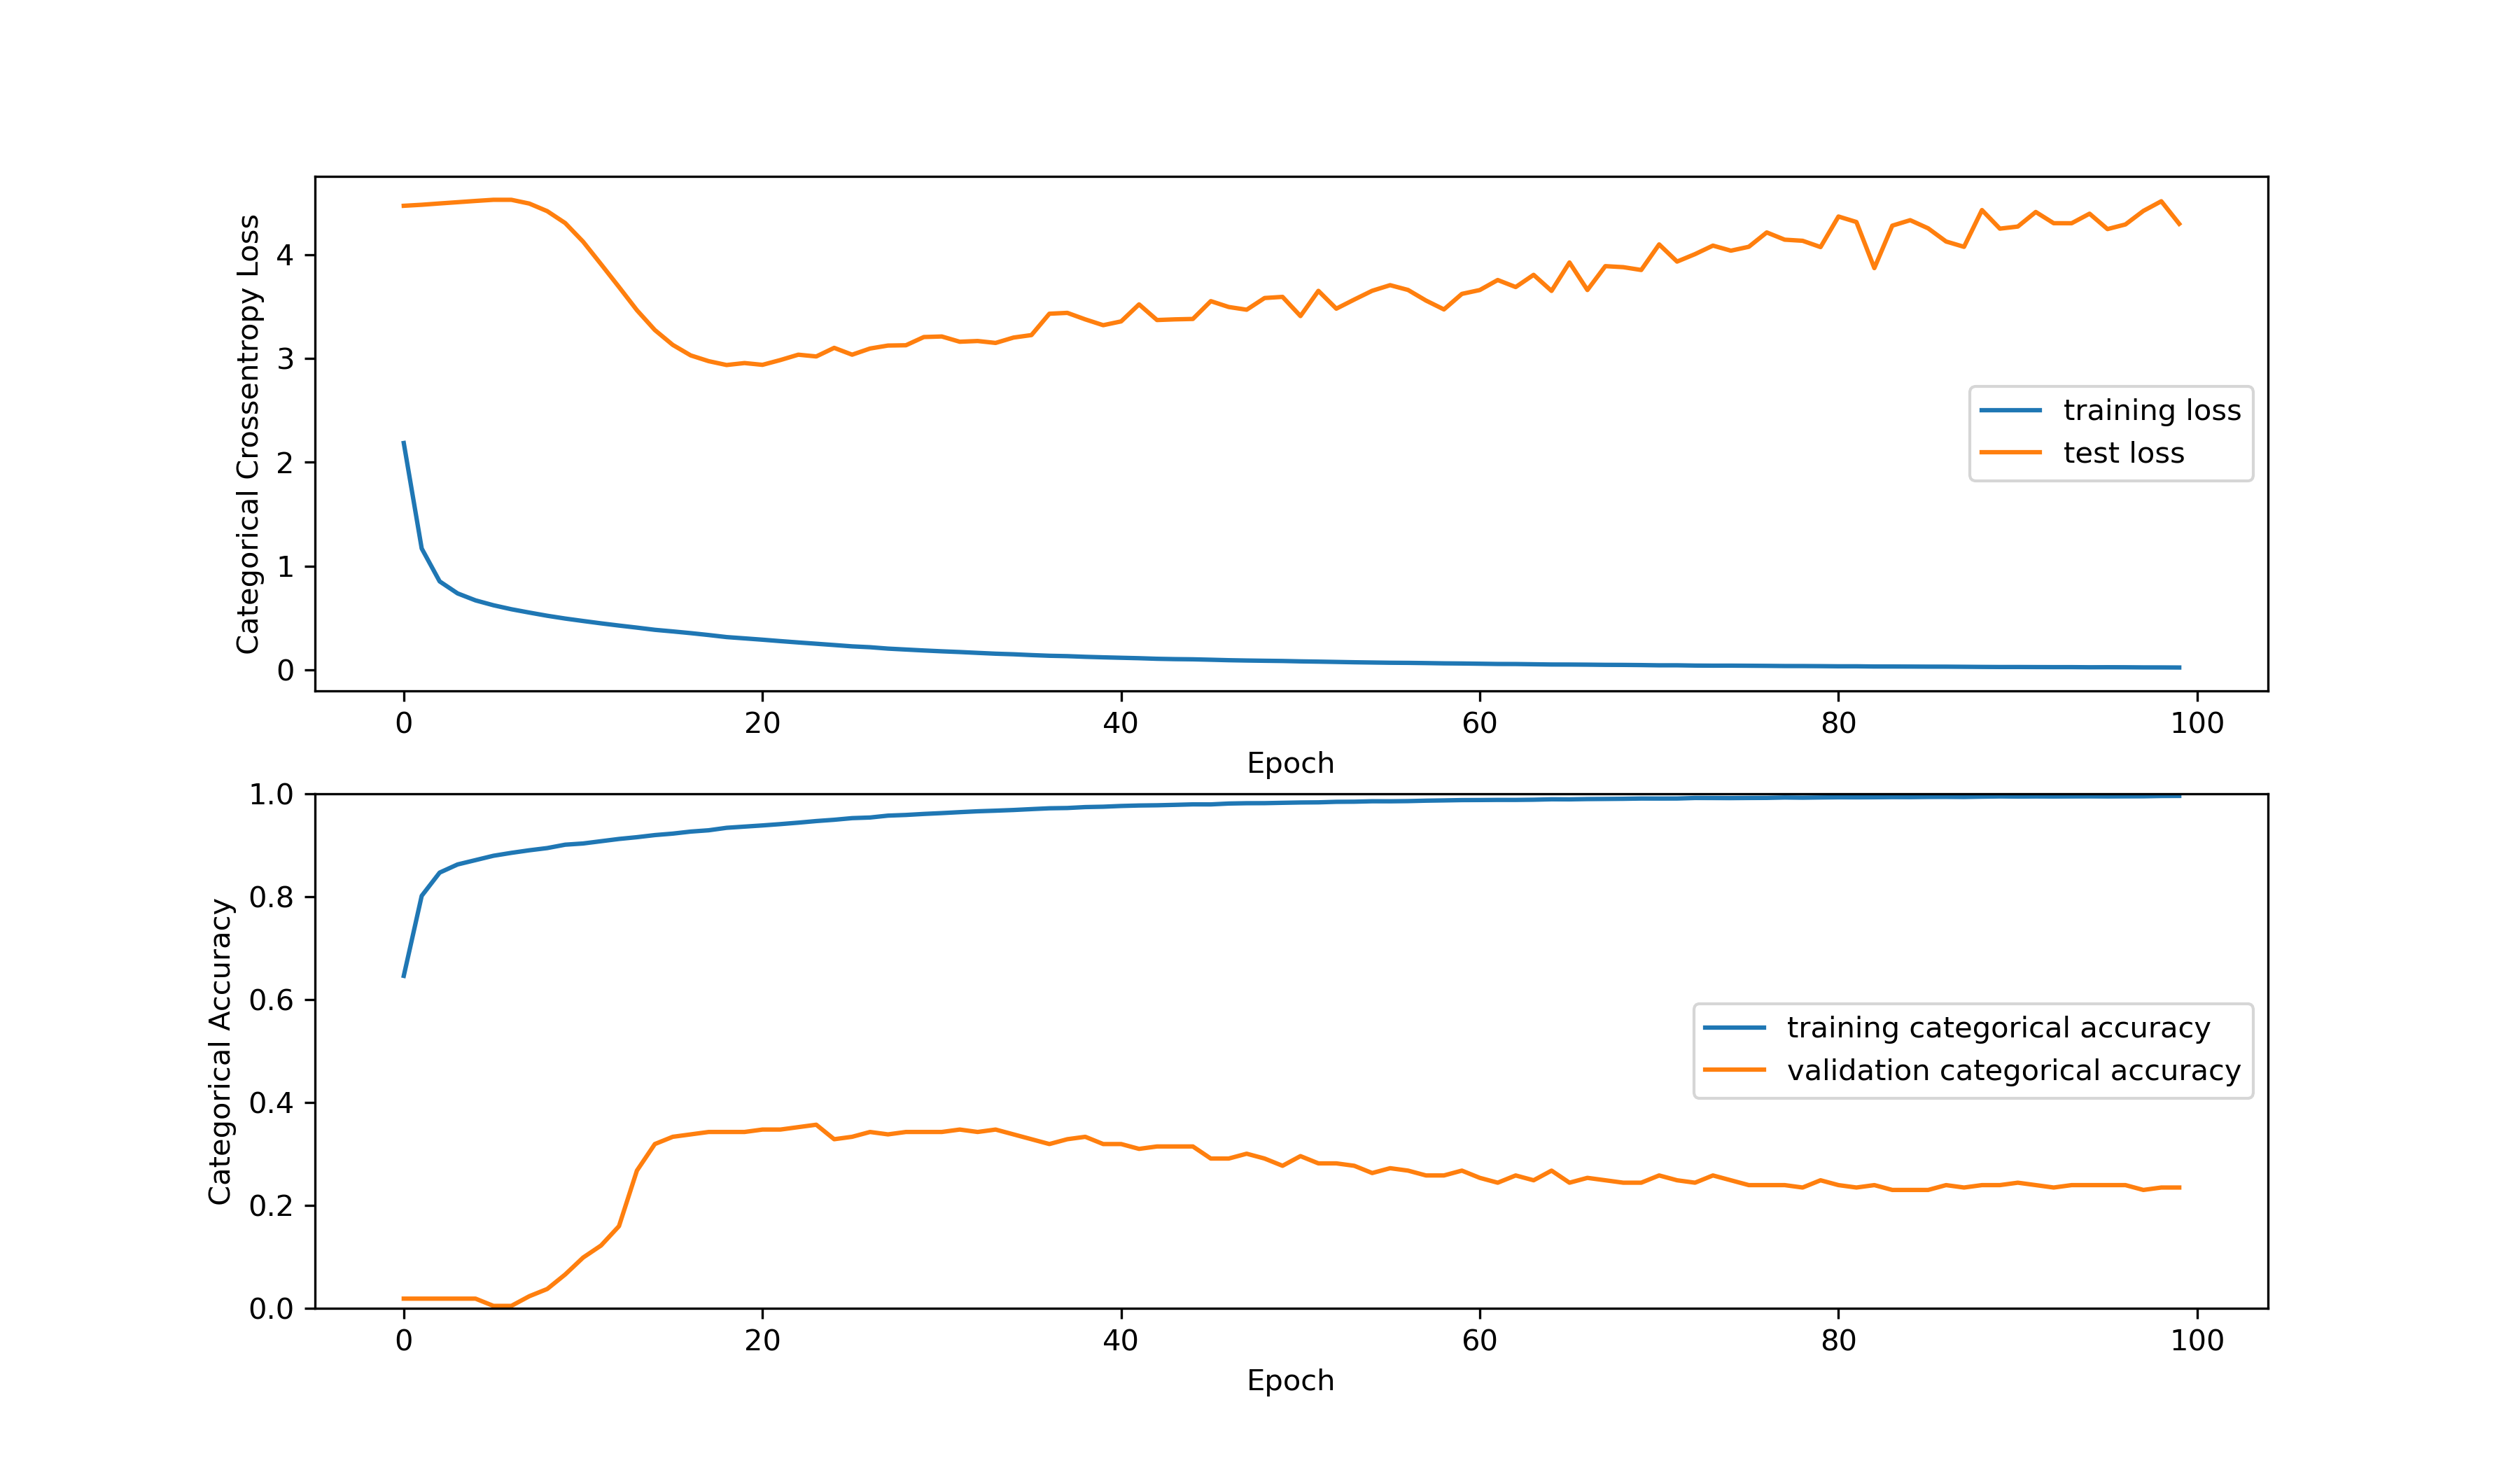
\includegraphics{Figures/overfit.png}
%       \caption{Overfit on the test data }
%       \label{fig:enter-label}
%   \end{figure}


\subsection{}
